\chapter{Конструкторский раздел}



\section{Основные концепции менеджера памяти}

В общем случае, эффективность менеджера памяти определяется следующими факторами:

\begin{enumerate}[label*=\arabic*.]
	\item \textbf{Задержка мутатора при выполнении операций выделения памяти и получения доступа к объектам.} При выполнении этих операций основная программа блокируется в ожидании обслуживания запроса к менеджеру памяти. Поэтому одной из его задач является минимизация времени блокировки мутатора.
	\item \textbf{Доля процессорного времени, затрачиваемая на сбор мусора.} Если сборщик мусора работает конкурентно с основной программой, то он отнимает процессорное время, выделенное программе операционной системой. Задачей сборщика является избежание ситуаций, при которых частая сборка мусора приводит к перегрузкам, замедляющим основную программу.
	\item \textbf{Накладные расходы памяти на хранение данных об обрабатываемых объектах.} Их минимизация повышает эффективность выделения памяти, однако, возможно, в ущерб трудоёмкости алгоритма сборки мусора.
	\item \textbf{Использование конкурентной сборки мусора.} Для снижения среднего времени паузы мутатора сборщик мусора может выполнять её конкурентно с потоками основной программы.
	\item \textbf{Использование параллельной сборки мусора.} Задействование сборщиком сразу нескольких потоков программы может ускорить его работу.
	\item \textbf{Использование алгоритма поколений.} Следование гипотезе поколений (см. п. \ref{generations}) позволяет снизить время одного цикла сборки мусора без потери её эффективности. Эффективность цикла сборки мусора можно оценить объёмом памяти, освобождённым за единицу времени.
\end{enumerate}

Целью разрабатываемого метода распределения памяти является минимизация нагрузки на мутатор за счёт использование параллельной и конкурентной сборки мусора.

Для организации объектов, обрабатываемых менеджером памяти, предлагается использовать модель поколений (см. п. \ref{generations}), предполагающей наличие молодого, промежуточного и старого поколения. Промежуточное поколение необходимо для того, чтобы замедлить продвижение объектов по поколениям. Если объект пережил один сбор мусора, то это не значит, что он будет жить дольше других объектов. А вот если он пережил два сбора мусора, то есть его возраст больше промежутка времени между сборами мусора, то вероятность его дальнейшего выживания оценивается выше.

Для реализации модели поколений куча разделяется на три пространства (поколения). Каждый новый объект помещается в первое поколение. Алгоритм сбора мусора выполняется только над объектами определённых поколений, и если объект не уничтожается во время обработки своего поколения, он будет перемещён в следующее поколение, где его будут анализировать реже. Если тот же объект не уничтожается после ещё одного цикла сборки мусора, он будет перемещен в последнее поколение, где его будут анализировать реже всего. Первоначально сборка мусора выполняется только в первом поколении. Такой подход позволяет сборщику мусора избежать сканирования всей кучи на каждом цикле сборки за счёт их разбиения на более короткие. В таком случае сборщик будет выполнять свою работу инкрементально, с каждым новым циклом увеличивая количество обрабатываемых объектов и охватывая более старые объекты.

Для контроля фрагментации кучи предлагается разделить пространство каждого поколения на \textbf{арены памяти} фиксированного размера, определяемого особенностями языка реализации. Предполагается, что именно арена будет являться единицей перераспределения памяти между поколениями. Это означает, что после циклов сборки мусора объекты будут перемещаться между аренами не по одному, а множеством. Такой подход позволит в некоторой степени сохранить эффективное расположение ссылок (см. п. \ref{reference_locality}).



\section{Проектирование алгоритмов работы с памятью}

\subsection{Представление дескриптора объекта}

Для управления объектами программы разрабатываемый менеджер памяти должен хранить следующие данные о них:

\begin{itemize}[label*=---]
	\item адрес для обеспечения доступа к объекту;
	\item метаданные о типе объекта для анализа его ссылок на другие объекты программы;
	\item арена памяти, в которой был выделен объект, для анализа загруженности арен;
	\item число ссылок на объект;
	\item данные о том, были ли финализированы все ссылки на объект;
	\item данные о том, участвует ли объект в цикле ссылок;
	\item идентификатор последнего цикла сборки мусора, в котором участвовал объект, для определения того, был ли размечен объект на текущем цикле сборки.
\end{itemize}

Также для избежания гонок данных при работе с дескриптором объекта он должен содержать примитив блокировки для осуществления атомарных операций над ним.

Для определения, является ли объект мусором, предлагается проверять следующие условия:

\begin{enumerate}[label*=\arabic*)]
	\item все ссылки на объект были финализированы;
	\item объект участвует в цикле ссылок и количество ссылок на него не превышает 1.
\end{enumerate}

Условие 1 не является достаточным для определения недостижимости объекта в основной программе, поскольку он может участвовать в цикле ссылок между мусорными объектами. В таком случае предлагается использование дизъюнкции условий 1 и 2 для определения достижимости объекта. Условие 1 соответствует состоянию счётчика ссылок на объект, а условие 2 предполагает осуществление трассирующей сборки мусора для определения циклических ссылок между объектами программы.

Стоит отметить, что ограничение по количеству ссылок на объект в условии 2 не даёт возможность идентифицировать мусорными те объекты, которые участвуют одновременно в нескольких циклах ссылок. Это означает, что сборщик мусора не сможет за один цикл сборки освободить все объекты, участвующие в пересекающихся циклах ссылок, опираясь на предположение о том, что подобные случаи будут встречаться в программах относительно редко. К тому же, для корректной идентификации объектов, участвующих в нескольких циклах ссылок, пришлось бы использовать алгоритмы обнаружения компонент сильной связности в орграфах, которые образуют объекты с помощью отношения ссылки. Примерами таких алгоритмов могут послужить алгоритмы Тарьяна и Косарайю \cite{graph_algorithms}. Их использование может существенно увеличить трудоёмкость алгоритмов сборки мусора.

\subsection{Алгоритм выделения памяти}

На рисунке \ref{fig:allocation} представлена схема алгоритма выделения памяти.

\begin{figure}[H]
	\centering
	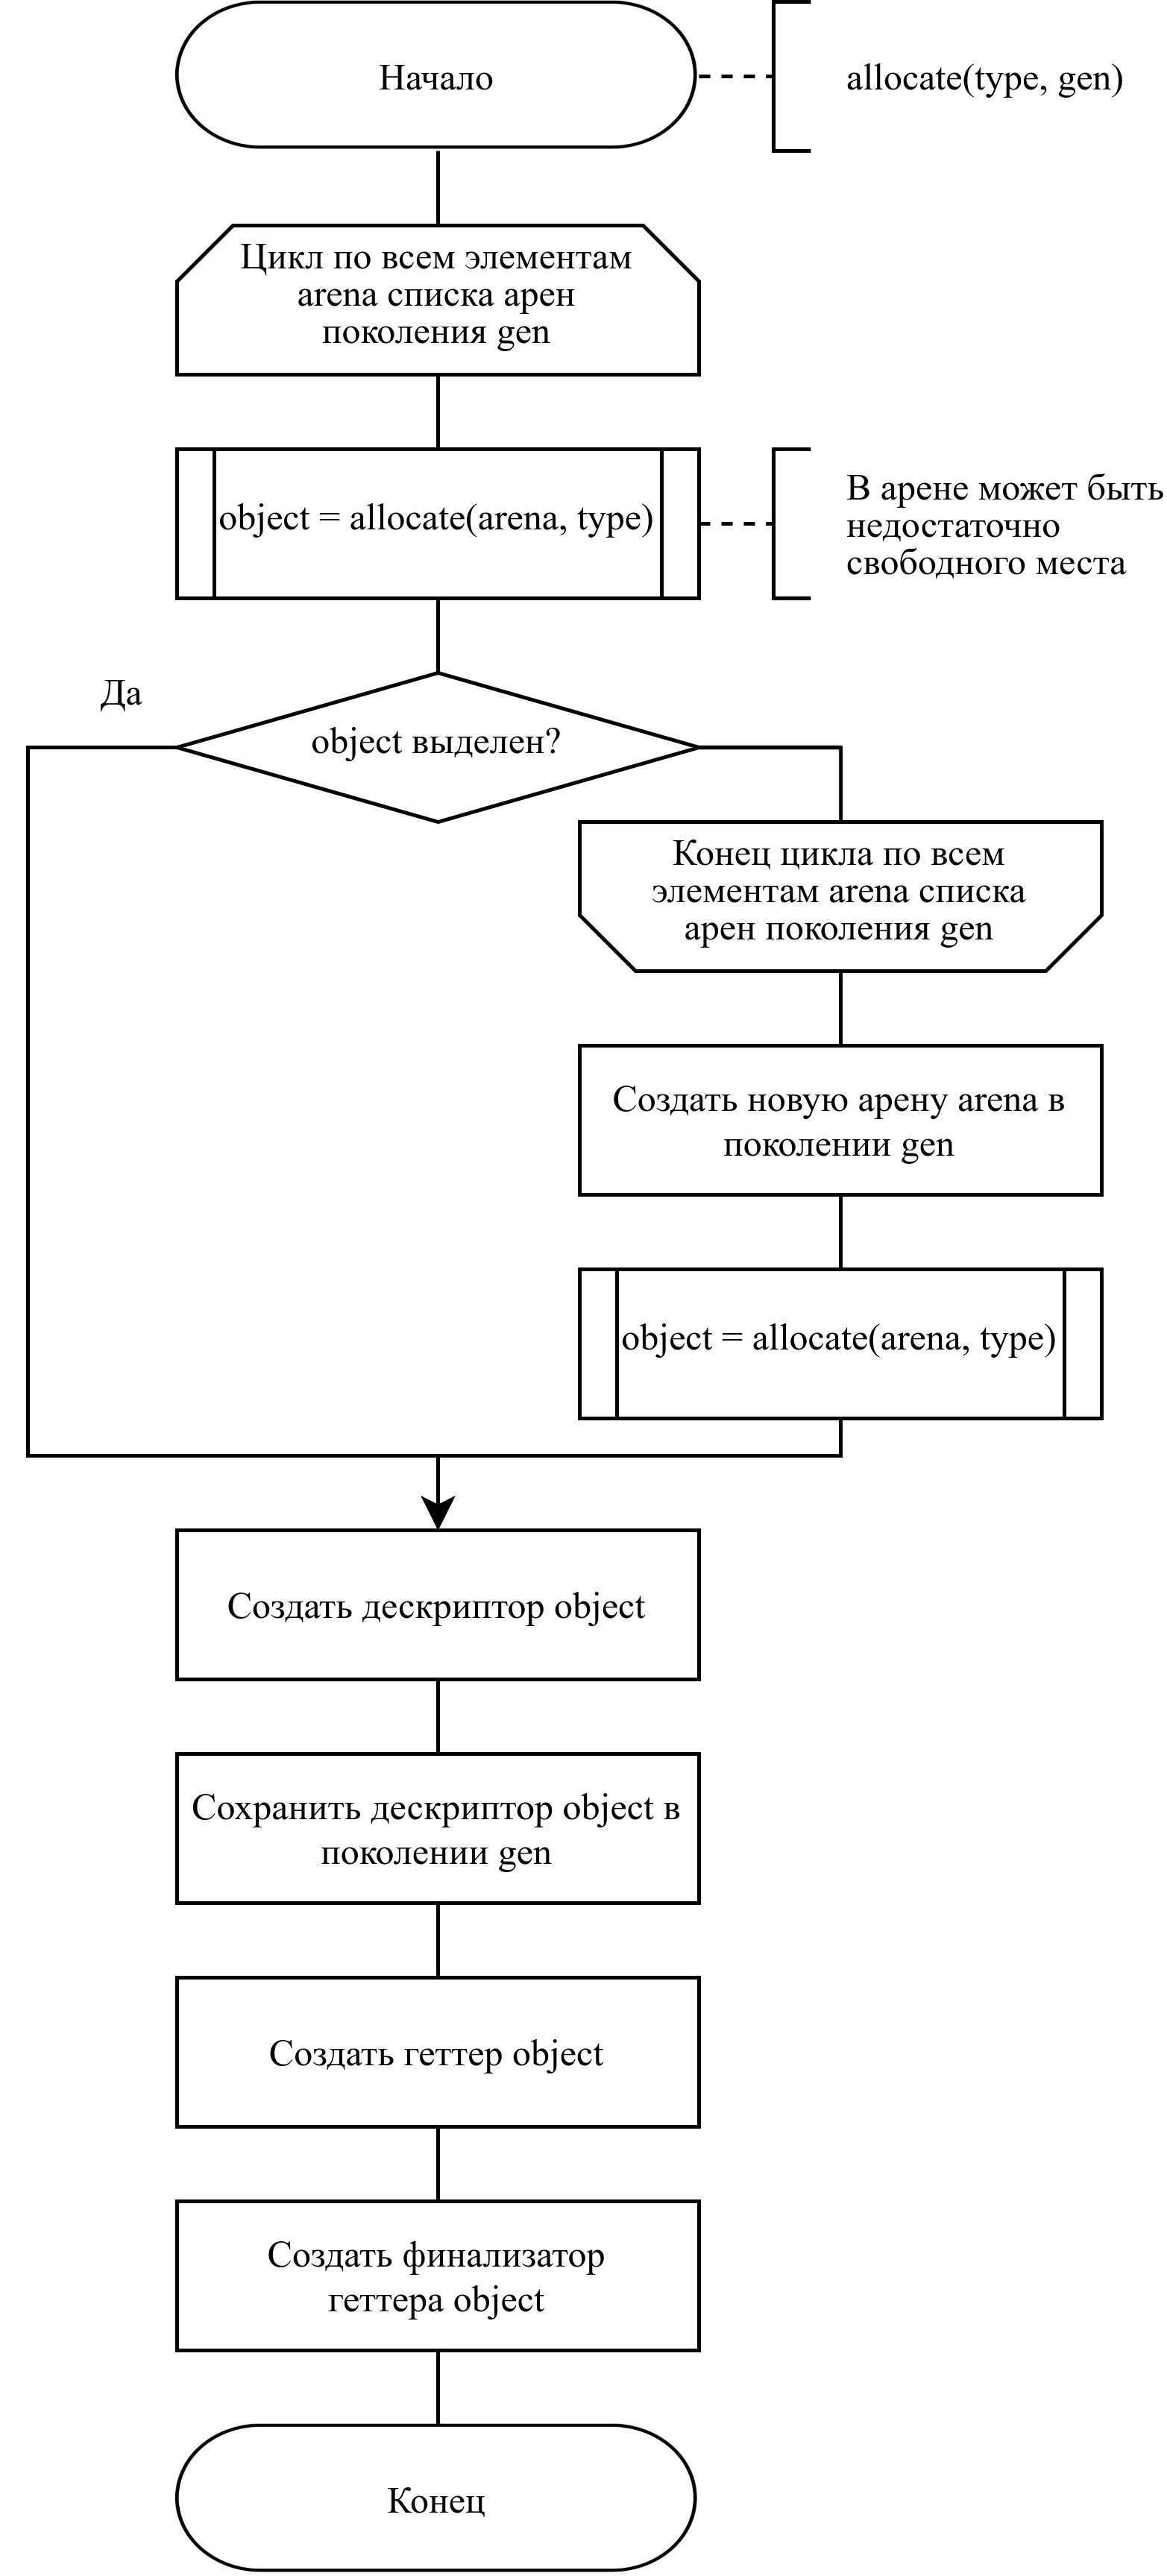
\includegraphics[height=0.95\textheight]{assets/allocate.png}
	\caption{Алгоритм выделения памяти}
	\label{fig:allocation}
\end{figure}

Геттер объекта является ссылкой на объект, поскольку предоставляет единственный вариант получения доступа к объекту из основной программы. Геттер можно считать барьером между основной программой и менеджером памяти, предотвращающим гонки данных.

Гарантия времени выполнения разрабатываемого метода подразумевает ограничение времени, которое пользовательская программа затрачивает на вызовы реализации метода, то есть на выделение памяти и обращение к выделенным объектам. Время выполнения обращения к объекту 

Дать асимптотическую оценку временной сложности алгоритма выделения

\subsection{Алгоритм освобождения памяти}

Инкрементальная сборка мусора

\subsection{Алгоритм сбора циклических ссылок}

+ условия его запуска

3 фазы: разметка, очистка и перераспределение объектов между поколениями



\section{Описание необходимых структур данных}



\section{Выбор подхода к реализации метода}

Обосновать в конструкторском разделе выбор между реализацией в виде модификации компилятора (можно вставлять кастомные барьеры чтения и записи (реализовываать их нативно), выполнять копирование и перемещение объектов, влиять на процесс разметки кучи + для сравнения методов не обязательно менять исходный код приложения и т.д.) и в виде подключаемой библиотеки: 
- нет лишней мишуры => работает быстрее
(ЦЕЛЬ ДИЗАЙНА РАЗРАБАТЫВАЕМОГО МЕНЕДЖЕРА ПАМЯТИ - МАКСИМАЛЬНО БЫСТРОЕ ВЫДЕЛЕНИЕ без лишней нагрузки на мутаторы)
- полностью заменить стандартный менеджер памяти своими патчами на компилятор нельзя, так как многие популярные библиотеки зависят от него => надо как-то уживаться с GC
- применимость на практике: подключить либу легче и удобнее, чем качать другой компилятор (по сути новый язык)

Нельзя безопасно обновлять указатели (?????), поэтому копировать объекты нельзя
+ Меньше накладных расходов
- Беды с фрагментацией

Описанные ранее алгоритмы работы менеджера памяти спроектированы таким образом, чтобы их выполнение можно было совмещать с работой сборщика мусора, встроенного в язык программирования реализации.



\section*{Выводы из конструкторской части}

В данном разделе были разработаны алгоритмы основные этапов метода автоматического управления памятью с гарантированным временем выполнения на основе подсчёта ссылок. Был описан подход к реализации метода.	

Исходя из количества данных, которые хранит в себе дескриптор объекта, можно выдвинуть предположение о том, что метод будет иметь наибольшую эффективность при его использовании для аллокации объектов программы, которые не содержат циклических ссылок и занимают объём памяти, намного превышающий размер дескриптора объекта. Тогда накладные расходы на хранение дескрипторов объектов и сборку циклических ссылок будут пренебрежимо малы по сравнению с ресурсными затратами основной программы.


